\input{../../main}

\begin{document}

\setphysstyle{ГЦФО 8}{Серия НТ-04}{03.10.2016}

\Large


\taskpic[7cm]{ Подсчитать полную минимальную работу, которую
  необходимо совершить, чтобы перекантовать ящик массой
  $m = 10^3 \mbox{ кг}$ сначала вокруг ребра $A_1B_1$, потом вокруг
  ребра $A_2B_2$. Длина ящика $l = 0,8 \mbox{ м}$, высота
  $h = 0,6 \mbox{ м}$. }{
  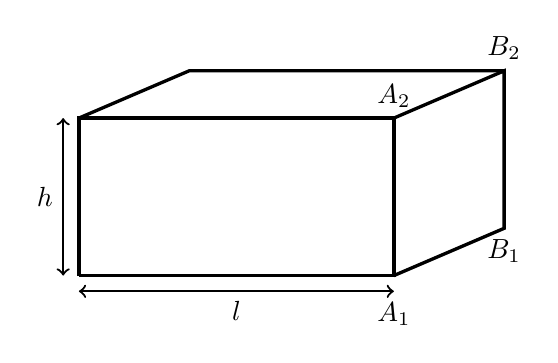
\begin{tikzpicture}
    \draw[very thick] (0, 2) -- ++ (1.4, 0.6) -- ++ (4, 0);
    \draw[very thick] (0, 0) -- ++ (4, 0) node[below=0.2cm] {$A_1$} -- ++ (0, 2)
    node[above,fill=white] {$A_{2}$} -- ++ (-4, 0) -- ++ (0, -2);
    \draw[very thick] (4, 0) -- ++ (1.4, 0.6) node[below] {$B_{1}$} -- ++ (0, 2)
    node[above] {$B_{2}$} -- ++ (-1.4, -0.6);
    \draw[thick,<->] (0, -0.2) -- ++ (4, 0) node[midway,below] {$l$};
    \draw[thick,<->] (-0.2, 0) -- ++ (0, 2) node[midway, left] {$h$};
  \end{tikzpicture}
}


\task{ На закрепленном вертикальном стержне навернута гайка. Гайку
  закрутили, так что она опустилась на расстояние $h$, совершив при
  этом работу $A_{1}$. Затем гайку открутили, так что она поднялась на
  высоту $h$, при этом была произведена работа $A_{2}$. Найдите массу
  гайки.  }


\task{ В результате измерения КПД двигателя получился равным
  $18\%$. Впоследствии выяснилось, что во время определения КПД часть
  топлива вытекала через прокладку. Какая часть топлива вытекала, если
  в исправном состоянии КПД двигателя равен $20\%$?}

\end{document}


%%% Local Variables: 
%%% mode: latex
%%% TeX-engine:xetex
%%% TeX-PDF-mode: t
%%% End:
